\subsection*{3.10 Magnetismus der Materie}
    Wird eine Materie mit magnetischen Eigenschaften in eine Induktionsspule eingefügt, so verstärkt sich die magnetische Wirkung um einen materialabhängigen Faktor $\mu$
    \mathbox{B_m = \mu \mu_0 H_0, L_m = \mu L_0}

    Magnetische Suszeptibilität:
    \mathbox{X = \mu - 1}

    Magnetisierung:
    \mathbox{\overrightarrow{M} = X \overrightarrow{H}}
    \begin{itemize}
        \item paramagnetische Materialien: $X > 0$, Magnetisierung in gleiche Richtung wie Feld. 
        \item diamagnetische Materialien: $X < 0$, Magnetisierung in entgegengesetzte Richtung wie Feld.
    \end{itemize}

    Elektronen bewegen sich auf einer Kreisbahn im Atom -> magnetisches Moment entsteht. Bei angelegtem magnetischem Feld werden die magnetischen Momente aller Atome parallel ausgerichtet
    \textbf{Schema mit magnetischem Moment einfügen}

    Hysterese: Wenn nach der Magnetisierung eines ferromagnetischen Materials das magnetische Feld wieder ausgeschalten wird, setzt ein "Memory-Effekt ein.
    Eine verbleibende magnetische Wirkung im Material bezeichnet man als \textbf{Remanenz}.
    Das Feld, welches benötigt wird, um die Remanenz auszulöschen, bezeichnet man als \textbf{Hoerzitivkraft}
    %\begin{figure}
        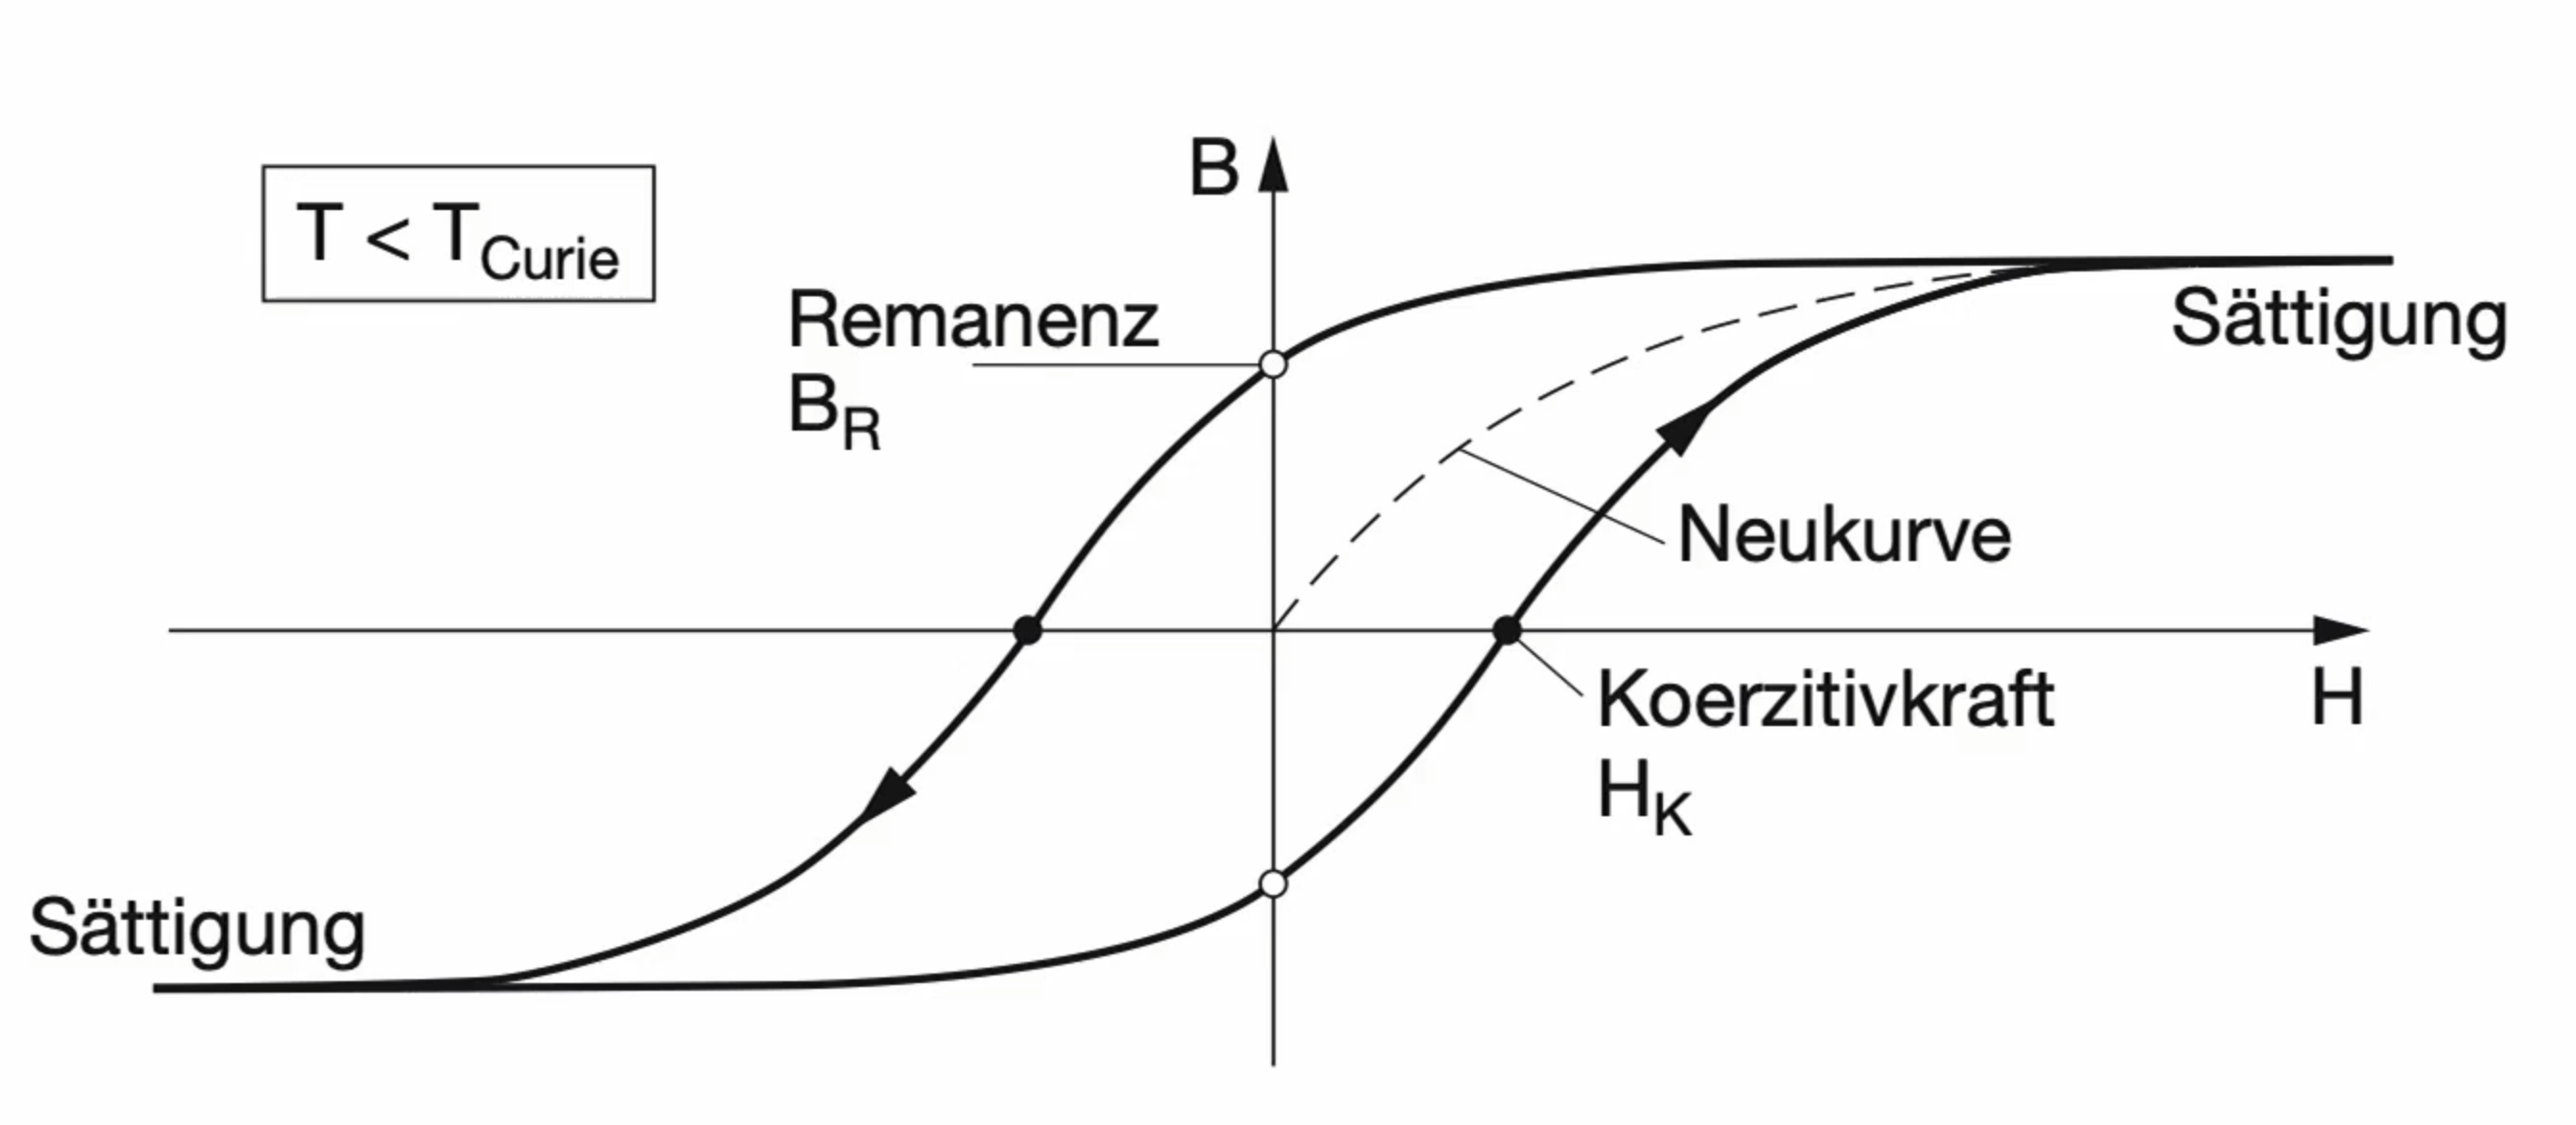
\includegraphics[height = 20mm]{src/images/permanentmagnet.png}
    %\end{figure}

    Meissner Effekt: Keine magnetischen Feldlinien treten in einen Supraleiter ein, perfektes diamagnetisches Verhalten.
    Anwendung: Magnet kann auf abgekühltem supraleiter-Material schweben, bsp. Magnetschwebebahn